\documentclass[lualatex,handout]{beamer}
\setbeamertemplate{footline}[frame number]
\usepackage{luatexja}
\usepackage{amsmath,amssymb}

%\usetheme{Berlin}
\usecolortheme{rose}

\usepackage{tikz}
\usepackage{pgfplots}
\pgfplotsset{compat=1.18}

%\usepackage[haranoaji]{luatexja-preset}
\usepackage[deluxe,ipaex]{luatexja-preset}
\renewcommand{\kanjifamilydefault}{\gtdefault}
%\setmainjfont{HaranoAjiGothic-Regular}

\usepackage{unicode-math}
%\setmathfont{Fira Math}
\setmathfont{STIX Two Math}
\setmathfont{STIX Two Math}[range=bfup/{Latin,latin,num,Greek,greek}]
\setmathfont{STIX Two Math}[range=bfit/{Latin,latin}]
\setmathfont{STIX Two Math}[range={"0000-"FFFF}]
\setmathrm{STIX Two Math}[StylisticSet=8]

%\usefonttheme{professionalfonts}

\usepackage{luacolor}

\newcommand{\mycolor}[2]{%
  \begingroup
  \colorlet{currentcolor}{.}%
  \color{#1}#2%
  \color{currentcolor}%
  \endgroup
}
\newcommand{\emm}[1]{\mycolor{red}{#1}}
\newcommand{\expt}[1]{\mathbb{E}\left[#1\right]}
\newcommand{\var}[1]{\mathbb{V}\left[#1\right]}
\newcommand{\cov}[1]{\mathsf{Cov}\left[#1\right]}
\newcommand{\vc}[1]{\mathsf{Var}\left[#1\right]}


\usepackage{xspace}
%\usepackage{bm}
%\newcommand\bm[1]{{\mathbf{#1}}}
\newcommand\dx{{\,\mathrm{d}x}}

\theoremstyle{definition}

\title{確率・統計基礎: 複数の確率変数、多変量正規分布}
\author{森 立平}
\date{}



\begin{document}
\begin{frame}[plain]
\maketitle
\end{frame}


\begin{frame}{複数の確率変数の確率密度関数}
\small
\begin{definition}
$p_{Z_1,\dotsc,Z_n}\colon \mathbb{R}\to\mathbb{R}$が
確率変数$Z_1,\dotsc,Z_n$の確率密度関数$\stackrel{\mathrm{def}}{\iff}$
\begin{align*}
\Pr(Z_1\le z_1, Z_2\le z_2,\dotsm Z_n\le z_n)&=
\int_{\substack{-\infty< x_1 \le z_1\\ -\infty< x_2\le z_2\\\vdots\\-\infty<x_n\le z_n}} p_{Z_1,\dotsc,Z_n}(x_1,x_2,\dotsc,x_n)\mathrm{d}{\symbf{x}_1^n}
\end{align*}
\end{definition}
%確率変数$Z_1,\dotsc,Z_n$が\emm{独立}のとき、
%\begin{align*}
%p_{Z_1,\dotsc,Z_n}(x_1,\dotsc,x_n)&=p_{Z_1}(x_1)p_{Z_2}(x_2)\dotsm p_{Z_n}(x_n)
%\end{align*}
%である。
一つの確率変数$Z_1$の確率密度関数は$\Pr(Z_1\le z_1) = \Pr(Z_1\le z_1, Z_2 <\infty,\dotsc, Z_n<\infty)$より
\begin{align*}
p_{Z_1}(x_1)&=
\int_{\substack{-\infty< x_s <\infty \;\forall s\ne 1}} p_{Z_1,\dotsc,Z_n}(x_1,x_2,\dotsc,x_n)\mathrm{d}{\symbf{x}_2^n}.
\end{align*}
他の$Z_k$の確率密度関数についても同様。
\end{frame}

\begin{frame}{独立確率変数}
\begin{align*}
\Pr(Z_1\le z_1, Z_2\le z_2,\dotsm Z_n\le z_n)&=
\Pr(Z_1\le z_1)\Pr(Z_2\le z_2)\dotsm \Pr(Z_n\le z_n)
\end{align*}
\begin{align*}
\int_{\substack{-\infty< x_1 \le z_1\\ -\infty< x_2\le z_2\\\vdots\\-\infty<x_n\le z_n}} p_{Z_1,\dotsc,Z_n}(x_1,x_2,\dotsc,x_n)\mathrm{d}{\symbf{x}_1^n}
&=
\end{align*}
\end{frame}

\begin{frame}{分散共分散行列}
\small
\begin{definition}[分散共分散行列]
確率変数$Z_1,\dotsc,Z_n$の\emm{分散共分散行列}(もしくは\emm{共分散行列})$\vc{\symbf{Z}}\in\mathbb{R}^{n\times n}$は
$(i,\,j)$成分に$\cov{Z_i,\,Z_j}=\expt{Z_iZ_j}-\expt{Z_i}\expt{Z_j}$を持つ行列である。
\end{definition}
\begin{align*}
\vc{\symbf{Z}}&=
\begin{bmatrix}
\var{Z_1}&\cov{Z_1,Z_2}&\cov{Z_1,Z_3}\\
\cov{Z_2,Z_1}&\var{Z_2}&\cov{Z_2,Z_3}\\
\cov{Z_3,Z_1}&\cov{Z_3,Z_2}&\var{Z_3}\\
\end{bmatrix}
\end{align*}
確率変数のベクトルや行列に対する$\expt{\cdot}$は成分毎に期待値を取ることを表す。
\begin{align*}
\symbf{Z} &= \begin{bmatrix}Z_1\\Z_2\\\vdots\\Z_n\end{bmatrix}&\text{とすると}\qquad
\expt{\symbf{Z}} &= \begin{bmatrix}\expt{Z_1}\\\expt{Z_2}\\\vdots\\\expt{Z_n}\end{bmatrix}
\end{align*}
である。
分散共分散行列は以下のように表せる。
\begin{align*}
\symbf{\Sigma}&=
\expt{\symbf{Z} \symbf{Z}^T} - \expt{\symbf{Z}}\expt{\symbf{Z}}^T
\end{align*}
\end{frame}

\begin{frame}{分散共分散行列の性質}
\begin{itemize}
\setlength{\itemsep}{2em}
\item $\vc{\symbf{Z}}$は対称行列である。
\item $\vc{\symbf{Z}}$は半正定値である。
\item $\vc{\symbf{Z}+\symbf{b}}=\vc{\symbf{Z}}$.
\item $\vc{A\symbf{Z}}=A\vc{\symbf{Z}}A^T$.
%\item $\vc{\symbf{Z}+\symbf{Y}}=\vc{\symbf{Z}} + \vc{\symbf{Y}} + $.
\end{itemize}
\end{frame}

\begin{frame}{線形変換の分散共分散行列}
行列$A\in\mathbb{R}^{m\times n}$と$n\times k$の確率変数行列$\symbf{Z}$について$\expt{A\symbf{Z}}=A\expt{\symbf{Z}}$である。
よって、$N$次元確率変数ベクトル$\symbf{Z}$について
\begin{align*}
&\expt{(\symbf{Z} - \expt{\symbf{Z}})(\symbf{Z} - \expt{\symbf{Z}})^T}\\
=&\expt{\symbf{Z}\symbf{Z}^T - \symbf{Z}\expt{\symbf{Z}}^T - \expt{\symbf{Z}}\symbf{Z}^T + \expt{\symbf{Z}}\expt{\symbf{Z}}^T}\\
=& \expt{\symbf{Z} \symbf{Z}^T} - \expt{\symbf{Z}}\expt{\symbf{Z}}^T
=\vc{\symbf{Z}}
\end{align*}
よって$\vc{\symbf{Z}+\symbf{b}}=\vc{\symbf{Z}}$である。

\vspace{1em}
\begin{align*}
\vc{A\symbf{Z}}&=\expt{\symbf{AZ} (\symbf{AZ})^T} - \expt{\symbf{AZ}}\expt{\symbf{AZ}}^T\\
&=A\expt{\symbf{Z} \symbf{Z}^T}A^T - A\expt{\symbf{Z}}\expt{\symbf{Z}}^TA^T\\
&=A\emm{\vc{\symbf{Z}}}A^T
\end{align*}
\end{frame}

\begin{frame}{分散共分散行列の半正定値性 I}
\small
\begin{align*}
&
\begin{bmatrix}
1&\expt{Z_1}&\expt{Z_2}&\expt{Z_3}\\
\expt{Z_1}&\expt{Z_1^2}&\expt{Z_1Z_2}&\expt{Z_1Z_3}\\
\expt{Z_2}&\expt{Z_2Z_1}&\expt{Z_2^2}&\expt{Z_2Z_3}\\
\expt{Z_3}&\expt{Z_3Z_1}&\expt{Z_3Z_2}&\expt{Z_3^2}\\
\end{bmatrix}\\
=&
\expt{
\begin{bmatrix}
1&Z_1&Z_2&Z_3\\
Z_1&Z_1^2&Z_1Z_2&Z_1Z_3\\
Z_2&Z_2Z_1&Z_2^2&Z_2Z_3\\
Z_3&Z_3Z_1&Z_3Z_2&Z_3^2\\
\end{bmatrix}}\\
=&
\expt{
\begin{bmatrix}
1\\
Z_1\\
Z_2\\
Z_3\\
\end{bmatrix}
\begin{bmatrix}
1&
Z_1&
Z_2&
Z_3
\end{bmatrix}}\ge 0\qquad (\text{半正定値行列の期待値は半正定値})
\end{align*}

任意の$\symbf{a}\in\mathbb{R}^n$ と$n\times n$半正定値ランダム行列$R$について
$\symbf{a}^T \expt{R}\symbf{a} = \expt{\symbf{a}^TR\symbf{a}}\ge 0$
なので$\expt{R}\ge0$.
\end{frame}

\begin{frame}{分散共分散行列の半正定値性 II}
\scriptsize
\begin{align*}
&
\begin{bmatrix}
-\expt{Z_1}&1&0&0\\
-\expt{Z_2}&0&1&0\\
-\expt{Z_3}&0&0&1\\
\end{bmatrix}
\begin{bmatrix}
1&\expt{Z_1}&\expt{Z_2}&\expt{Z_3}\\
\expt{Z_1}&\expt{Z_1^2}&\expt{Z_1Z_2}&\expt{Z_1Z_3}\\
\expt{Z_2}&\expt{Z_2Z_1}&\expt{Z_2^2}&\expt{Z_2Z_3}\\
\expt{Z_3}&\expt{Z_3Z_1}&\expt{Z_3Z_2}&\expt{Z_3^2}\\
\end{bmatrix}\\
=&
\begin{bmatrix}
0&\expt{Z_1^2}-\expt{Z_1}^2&\expt{Z_1Z_2}-\expt{Z_1}\expt{Z_2}&\expt{Z_1Z_3}-\expt{Z_1}\expt{Z_3}\\
0&\expt{Z_2Z_1}-\expt{Z_2}\expt{Z_1}&\expt{Z_2^2}-\expt{Z_2}^2&\expt{Z_2Z_3}-\expt{Z_2}\expt{Z_3}\\
0&\expt{Z_3Z_1}-\expt{Z_3}\expt{Z_1}&\expt{Z_3Z_2}-\expt{Z_3}\expt{Z_2}&\expt{Z_3^2}-\expt{Z_3}^2\\
\end{bmatrix}\\
\end{align*}
\begin{align*}
&
\begin{bmatrix}
0&\var{Z_1}&\cov{Z_1, Z_2}&\cov{Z_1, Z_3}\\
0&\cov{Z_2, Z_1}&\var{Z_2}&\cov{Z_2, Z_3}\\
0&\cov{Z_3, Z_1}&\cov{Z_3, Z_2}&\var{Z_3}
\end{bmatrix}
\begin{bmatrix}
-\expt{Z_1}& -\expt{Z_2}& -\expt{Z_3}\\
1&0&0\\
0&1&0\\
0&0&1\\
\end{bmatrix}\\
&=\vc{\symbf{Z}}
\end{align*}

$A\ge 0$のとき任意の行列$B$について$BAB^T\ge 0$なので$\vc{\symbf{Z}}\ge 0$である。
\end{frame}

\begin{frame}{多変量正規分布}
\begin{definition}[多変量正規分布]
確率変数$Z_1,\dotsc,Z_n$が平均$\symbf{\mu}\in\mathbb{R}^n$、分散共分散行列$\Sigma\in\mathbb{R}^{n\times n}$の多変量正規分布は確率密度関数
\begin{align*}
p_{\symbf{Z}}(\symbf{x}) &= \frac1{\sqrt{(2\pi)^n\det(\Sigma)}} \mathrm{e}^{-\frac12 (\symbf{x}-\symbf{\mu})^T\Sigma^{-1} (\symbf{x}-\symbf{\mu})}
\end{align*}
で定義される。
\end{definition}
\end{frame}

\begin{frame}{密度関数の積分}
\small
多変量正規分布の密度関数を積分して1になることを確認する。
$\Sigma$は対称行列なのである直交行列$V$と対角行列$D$が存在して$\Sigma=V^TDV$と表せる(スペクトル分解)。
また$\Sigma$は正定値なので、$D$の対角成分は正である。
\begin{align*}
&\int_{\mathbb{R}^n} \frac1{\sqrt{(2\pi)^n\det(\Sigma)}} \mathrm{e}^{-\frac12 (\symbf{x}-\symbf{\mu})^T\Sigma^{-1} (\symbf{x}-\symbf{\mu})}\mathrm{d}x\\
&=
\int_{\mathbb{R}^n} \frac1{\sqrt{(2\pi)^n\det(\Sigma)}} \mathrm{e}^{-\frac12 \symbf{x}^T\Sigma^{-1} \symbf{x}}\mathrm{d}x\\
&=
\int_{\mathbb{R}^n} \frac1{\sqrt{(2\pi)^n\det(D)}} \mathrm{e}^{-\frac12 (V\symbf{x})^TD^{-1} (V\symbf{x})}\mathrm{d}x\qquad(\Sigma=V^TDV)\\
&=
\int_{\mathbb{R}^n} \frac1{\sqrt{(2\pi)^n\det(D)}} \mathrm{e}^{-\frac12 \symbf{y}^TD^{-1} \symbf{y}}\frac1{|\det(V)|}\mathrm{d}y\qquad (y=Vx)\\
&=
\int_{\mathbb{R}^n} \frac1{\sqrt{(2\pi)^n\det(D)}} \mathrm{e}^{-\frac12 \symbf{z}^T \symbf{z}}\frac1{|\det(\sqrt{D^{-1}})|}\mathrm{d}z\qquad (z=\sqrt{D^{-1}}y)\\
&=
\int_{\mathbb{R}^n} \frac1{\sqrt{(2\pi)^n}} \mathrm{e}^{-\frac12 \symbf{z}^T \symbf{z}}\mathrm{d}z
=\prod_{k=1}^n\left(\int_{-\infty}^\infty \frac1{\sqrt{2\pi}}\mathrm{e}^{-\frac{z_k^2}2}\mathrm{d}z_k\right) = 1
\end{align*}
\end{frame}

\begin{frame}{多変数の特性関数}
\begin{definition}[多変数特性関数]
$n$次元確率変数$X$の\emm{特性関数}$\varphi_{X}\colon\mathbb{R}^n\to\mathbb{C}$を以下で定義する。
\begin{align*}
\varphi_{X}(t) &:= \expt{\mathrm{e}^{i\langle t,\, X\rangle}}.
\end{align*}
ここで$\langle t,\, X\rangle := \sum_{k=1}^n t_k X_k$である。
\end{definition}

\vspace{1em}
$X$と$Y$の分布が同じ$\emm{\iff}\varphi_X=\varphi_Y$ (ルベーグ積分に基づいた議論が必要).

\vspace{1em}
%$X$が$k$次モーメントを持つ$\iff$$\varphi_X$は0で$k$回微分できる。
\begin{align*}
%\left.\frac{\mathrm{d}^k\varphi_X(t)}{\mathrm{d}t^k}\right|_{t=0} &= i^k \expt{X^k}.
\left.\frac{\partial \varphi_X(t)}{\partial t_k}\right|_{t=0} &= \left.\expt{iX_k\mathrm{e}^{i\langle t,\, X\rangle}}\right|_{t=0} = i\expt{X_k}\\
\left.\frac{\partial^2 \varphi_X(t)}{\partial t_k\partial t_\ell}\right|_{t=0} &= \left.\expt{(iX_k)(iX_\ell)\mathrm{e}^{i\langle t,\, X\rangle}}\right|_{t=0} = -\expt{X_kX_\ell}.
\end{align*}
\end{frame}

\begin{frame}{多変数の特性関数の性質}
\begin{itemize}
\setlength{\itemsep}{1em}
\item $\varphi_{X+b}(t) = \varphi_X(t)\mathrm{e}^{i\langle t,\, b\rangle}\qquad\forall b\in\mathbb{R}^n$.
\item $\varphi_{AX}(t) = \varphi_X(A^Tt)\qquad\forall A\in\mathbb{R}^{m\times n}$.
\item $\varphi_{X+Y}(t) = \varphi_X(t)\varphi_Y(t)$.
\end{itemize}
\end{frame}

\begin{frame}{多変量正規分布の特性関数}
\small
\begin{align*}
&\expt{\mathrm{e}^{i\langle t,\,X\rangle}}\\
&=\int_{-\infty}^\infty \frac1{\sqrt{(2\pi)^n\det(\Sigma)}} \mathrm{e}^{-\frac12 (\symbf{x}-\symbf{\mu})^T\Sigma^{-1} (\symbf{x}-\symbf{\mu})}\mathrm{e}^{i\langle t,\, x\rangle}\mathrm{d}x\\
&= \int_{-\infty}^\infty \frac1{\sqrt{(2\pi)^n\det(\Sigma)}} \mathrm{e}^{-\frac12 \langle\Sigma^{-\frac12}(x-\mu),\,\Sigma^{-\frac12}(x-\mu)\rangle+i\langle \Sigma^{\frac12}t,\, \Sigma^{-\frac12}x\rangle}\mathrm{d}x\\
&= \int_{-\infty}^\infty \frac1{\sqrt{(2\pi)^n\det(\Sigma)}} \mathrm{e}^{-\frac12 \langle\Sigma^{-\frac12}(x-\mu-i\Sigma t),\,\Sigma^{-\frac12}(x-\mu-i\Sigma t)\rangle +i\langle \mu,\, t\rangle - \frac12\langle \Sigma^\frac12t,\,\Sigma^\frac12t\rangle}\mathrm{d}x\\
&= \mathrm{e}^{i\langle \mu,\, t\rangle - \frac12\langle \Sigma^\frac12t,\,\Sigma^\frac12t\rangle}
\end{align*}
\begin{align*}
\left.\frac{\partial \varphi_Z(t)}{\partial t_k}\right|_{t=0} &= i\mu_k\\
\left.\frac{\partial^2 \varphi_Z(t)}{\partial t_k\partial t_\ell}\right|_{t=0} &= 
\end{align*}
\end{frame}

\begin{frame}{多変量正規分布の一次変換}
\begin{lemma}
$n$次元の確率変数$\symbf{Z}\sim N(\symbf{\mu}, \Sigma)$のとき、
$A\symbf{Z}+\symbf{b}\sim N(A\symbf{\mu}+\symbf{b}, A\Sigma A^T)$.
%$Z_k\sim N(\mu_k, \Sigma_{k,k})$.
\end{lemma}
\begin{proof}
$\varphi_Z(t) = \mathrm{e}^{i\langle \mu,\, t\rangle - \frac12\langle \Sigma^\frac12t,\,\Sigma^\frac12t\rangle}$より、
\begin{align*}
\varphi_{AZ+b}(t) &= \varphi_{AZ}(t)\mathrm{e}^{i\langle t,\,b\rangle} = \varphi_Z(A^Tt)\mathrm{e}^{i\langle t,\,b\rangle}\\
&= \mathrm{e}^{i\langle \mu,\, A^T t\rangle - \frac12\langle \Sigma^\frac12A^T t,\,\Sigma^\frac12A^T t\rangle + i\langle t,\,b\rangle}\\
&= \mathrm{e}^{i\langle A\mu,\, t\rangle - \frac12\langle \Sigma^\frac12A^T t,\,\Sigma^\frac12A^T t\rangle+ i\langle t,\,b\rangle}\\
&= \mathrm{e}^{i\langle A\mu + b,\, t\rangle - \frac12\langle \Sigma^\frac12A^T t,\,\Sigma^\frac12A^T t\rangle}
\end{align*}
これは$N(A\mu+b,\, A\Sigma A^T)$の特性関数である。
\end{proof}
\end{frame}

\begin{frame}{多変量正規分布$\to$1変数正規分布}

\end{frame}

\begin{frame}{確率密度関数}
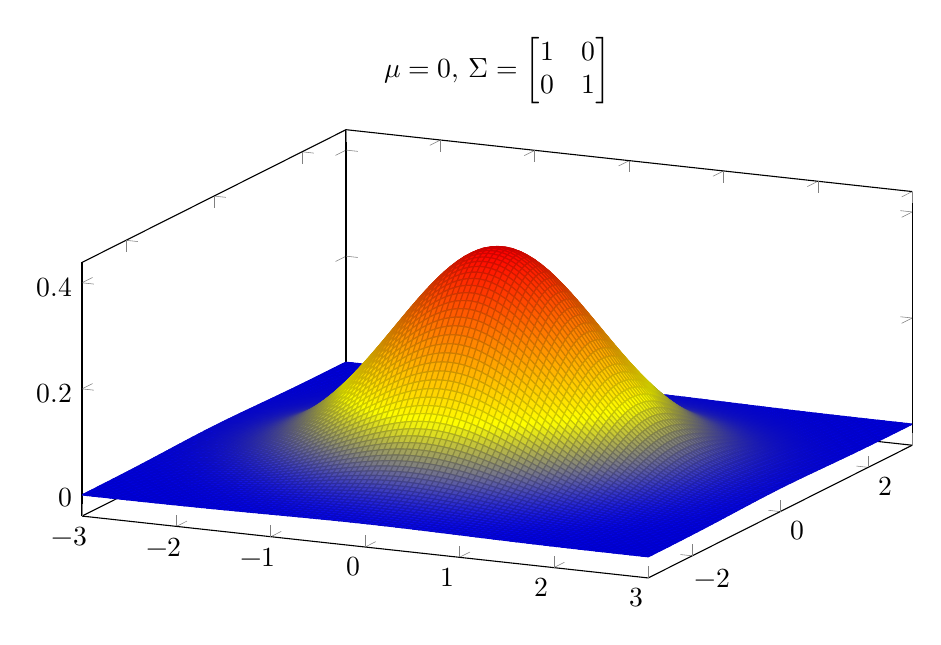
\begin{tikzpicture}
\begin{axis}[
%    title={$\frac1{2\pi}\mathrm{e}^{-\frac12(x^2+y^2)}$},
    title={$\mu=0,\,\Sigma = \begin{bmatrix}1&0\\0&1\end{bmatrix}$},
    width=\textwidth, height=\axisdefaultheight,
%%    zlabel={$p(x,y)$},
%    xlabel={$x$},
%    ylabel={$y$},
%    xmin=-3, xmax=3,
%    ymin=-3, ymax=3,
%    scaled ticks = false,
%    isosamples=100,
%    pm3d = true
    %tick label style={/pgf/number format/assume math mode=true, font=\footnotesize\sffamily},
    %yticklabel style={/pgf/number format/.cd, fixed, fixed zerofill, precision=2},
    %    domain=0:\binomN,samples at={0,1,...,\binomN},
    %mark options={scale=0.75, blue},
    %ybar, bar width = .75pt
        ]
%\addplot[ycomb] {binom(x,\binomN,0.3)};
%\addplot {binom(x,\binomN,0.3)};
\addplot3[surf, domain=-3:3, samples=100] {1.0/sqrt(2*pi) * exp(-0.5*(x^2 + y^2))};
\end{axis}
\end{tikzpicture}
\end{frame}

\begin{frame}{確率密度関数}
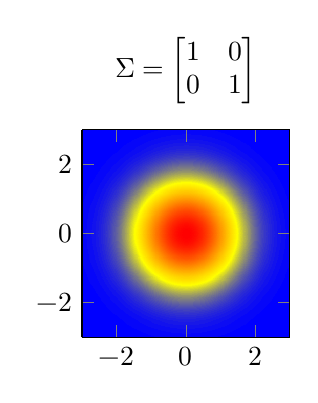
\begin{tikzpicture}
\begin{axis}[
    title={$\Sigma = \begin{bmatrix}1&0\\0&1\end{bmatrix}$},
    width=120, height=120,
    view={0}{90},
    %colorbar horizontal
        ]
\addplot3[contour filled={number=128}, domain=-3:3, samples=100] {1.0/sqrt(2*pi) * exp(-0.5*(x^2 + y^2))};
\end{axis}
\end{tikzpicture}
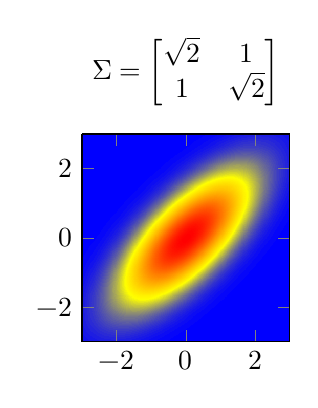
\begin{tikzpicture}
\begin{axis}[
    title={$\Sigma = \begin{bmatrix}\sqrt{2}&1\\1&\sqrt{2}\end{bmatrix}$},
    width=120, height=120,
    view={0}{90},
    %colorbar horizontal
        ]
\addplot3[contour filled={number=128}, domain=-3:3, samples=100] {1.0/sqrt(2*pi) * exp(-0.5*(sqrt(2)*x^2 + sqrt(2)*y^2 - 2*x*y))};
\end{axis}
\end{tikzpicture}
%
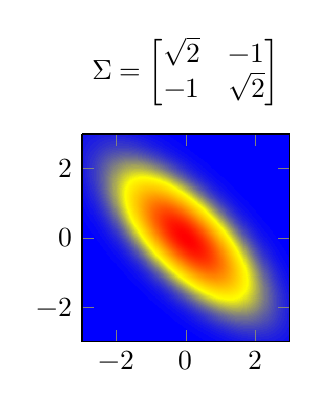
\begin{tikzpicture}
\begin{axis}[
    title={$\Sigma = \begin{bmatrix}\sqrt{2}&-1\\-1&\sqrt{2}\end{bmatrix}$},
    width=120, height=120,
    view={0}{90},
    %colorbar horizontal
        ]
\addplot3[contour filled={number=128}, domain=-3:3, samples=100] {1.0/sqrt(2*pi) * exp(-0.5*(sqrt(2)*x^2 + sqrt(2)*y^2 + 2*x*y))};
\end{axis}
\end{tikzpicture}
\end{frame}

\end{document}
